\documentclass[11pt]{article}
\usepackage{amsmath}
\usepackage{amssymb}
\usepackage{graphicx}
\usepackage{nips15submit_e, times}
\usepackage[T1]{fontenc}

\title{Midway Report: Semi-Supervised Learning of Pen-Based OCR.}
\author{Joshua Brakensiek, Jacob Imola, Sidhanth Mohanty}

\begin{document}

\maketitle

\begin{abstract}

  This report explores using semi-supervised learning to classify vector-based representations of handwritten digits. We describe related semi-supervised approaches such as transductive support vector machines (TSVMs). We present our latest progress on the project, including a baseline approach using TSVMs. We then outline our future work.

\end{abstract}



\newcommand{\Seq}{\operatorname{Seq}}

\section{Background}

Handwriting recognition is a classic machine learning problem. Generally, an image of a digit is inputted to an algorithm and classified. Instead of taking this approach, we used the sets,  ``Pen-Based Recognition of Handwritten Digits Data Set'' \cite{Alpaydin:1998} from the UCI Machine Learning Repository \cite{Lichman:2013}, which consist of pixel coordinates that the writers' pens took at certain time intervals. This data set, which has over 10,000 data points, consists entirely of drawings of the digits $0, \hdots, 9$. We seek to explore if adding the extra information of time while sacrificing some detail from the shape of the digits can produce a viable semi-supervised model.  We implement our learning algorithms in Python 2.7, using on the NumPy, SciPy, and Scikit-learn libraries (and possibly other libraries as we see fit). The models we try are Transductive Support Vector Machines and graph-based kernel methods and regularization. Throughout this paper, let $X = \{x_1, x_2, \ldots, x_k\}$ be the labeled training data, $Y = \{y_1, y_2, \ldots, y_k\}$ be the corresponding labels, $X^* = \{x^*_1, x^*_2, \ldots, x^*_n$ be the unlabeled training data, and $Y^* = \{y^*_1, y^*_2, \ldots, y^*_n$ be variables representing the unlabeled training data's labels. Now, we will give a description of the models: \par

Recall that an SVM reduces to the following primal problem:

\begin{equation}\label{eq:1}
\arg\min_{w, b, \zeta} \frac{1}{2}w^Tw+C\sum_{i=1}^k\zeta_i
\end{equation}

\begin{align*}
\textrm{subject to}\quad \forall_{i=1}^k&: y_i(wx_i+b)\geq 1-\zeta_i \\
\forall_{i=1}^k&: \zeta_i>0
\end{align*}

A TSVM's primal problem allows the unlabeled data to take on any label, and hence reduces to a similar problem \cite{Joachims:1999}:

\begin{equation}\label{eq:2}
\arg\min_{w, b, \zeta, \zeta^*, Y^*} \frac{1}{2}w^Tw+C\sum_{i=1}^k\zeta_i+C^*\sum_{i=1}^n\zeta^*_i
\end{equation}

\begin{align*}
\textrm{subject to}\quad \forall_{i=1}^k&: y_i(wx_i+b)\geq 1-\zeta_i \\
\forall_{i=1}^n&: y^*_i(wx^*_i+b)\geq 1-\zeta^*_i \\
\forall_{i=1}^k&: \zeta_i>0 \\
\forall_{i=1}^n&: \zeta^*_i>0
\end{align*}

Here, $C$ and $C^*$ are parameters that control the type of fit we get.

\section{Related Work}

The TSVM algorithm that we implemented requires that in the unlabeled
data, the number of data points classified is constrained to be
exactly equal to some parameter $num_+$. \cite{joachims2003transductive}
shows that this special kind of TSVM is equivalent to solving
a $s$-$t$ min cut problem, where the size of the partitions are fixed beforehand, and explores an algorithm called spectral graph transducer,
that does not require the sizes of the partitions to be fixed beforehand.

Closely related to the graph interpretation of semi-supervised SVMs
are methods intersecting at spectral graph theory and semi-supervised
learning like Laplacian SVMs and Manifold regularization
(see \cite{belkin2005manifold}). This method assume a distribution $P$
over $X\times \mathbb{R}$ from which labeled examples $(x,y)$ are drawn,
and assumes that the marginal distribution of $P$ on $X$, denoted $P_X$,
has the structure of a Riemannian manifold and uses this model
as a basis for a family of methods.

Another related semi-supervised learning technique that could
be applied to TSVMs is co-training, introduced in
\cite{blum1998combining}. This technique splits each unlabeled
example into multiple `views' (an example as specified in \cite{blum1998combining} would be how webpages can be partitioned into
the content on that page and content on other pages that link to it),
and two learning algorithms are trained on different views. Then,
the labels provided by the algorithms on previously unlabeled examples
are used to increase the labeled data available to the other
algorithm to train on.

\cite{joachims1999making} describes an algorithm called $SVM^{light}$,
which is faster than traditional algorithms for training
semi-supervised SVM that scales well with a large amount of
data, but sacrifices on accuracy.

\section{Methods}

\subsection{TSVM}

One TSVM method we use is an SVM with local search which was first described in \cite{Joachims:1999}. We use a more generalized version of an SVM:
\begin{equation}\label{eq:3}
\arg\min_{w, b, \zeta,\zeta^*} \frac{1}{2}w^Tw+C\sum_{i=1}^k\zeta_i+C^*_+\sum_{i=1}^n\zeta^*_i[y^*_i == 1]+C^*_-\sum_{i=1}^n\zeta^*_i[y^*_i == -1]
\end{equation}

\begin{align*}
\textrm{subject to}\quad \forall_{i=1}^k&: y_i(wx_i+b)\geq 1-\zeta_i \\
\forall_{i=1}^n&: y^*_i(wx^*_i+b)\geq 1-\zeta^*_i \\
\forall_{i=1}^k&: \zeta_i>0 \\
\forall_{i=1}^n&: \zeta^*_i>0
\end{align*}

Let's denote an SVM with such an objective function as $SVM(C,C^*_+,C^*_-,T^*)$.
The user inputs $C$ and $C^*$ defined in (\ref{eq:2}) and two additional parameters: $num_+$, which is the number of $Y^*$ that will be equal to 1, and $\epsilon$ which is a weight to be used later. First, a regular SVM is trained with $X$, $Y$, and $C$, using the objective function of (\ref{eq:1}), and we find the margin distances of $X^*$. We take the $num_+$ most positive margin distances and classify them as 1 in $Y^*$. Then, we initialize two weights, $C^*_- = \epsilon$ and $C^*_+$ such that $\frac{C^*_+}{C^*_-} = \frac{num_+}{n-num_+}$. Then, we call $SVM(C,C^*_+,C^*_-,Y^*)$, and we greedily find two indices $i$ and $j$ such that $y^*_j = -y^*_i$, $\zeta^*_i > 0$ and $\zeta^*_j > 0$ and $\zeta^*_i+\zeta^*_j > 2$, then we know that flipping $y^*_i$ and $y^*_j$ will reduce (\ref{eq:3}) and preserve the number of positive $num_+$ examples. We do this as much as possible, and then set $C^*_+ = \max\{2C^*_+, C^*_+\}$ and $C^*_- = \max\{2C^*_-, C^*_-\}$. This increases the importance of the unlabeled data, because its label accuracy should be increasing. Finally, we call $SVM(C,C^*_+,C^*_-,Y^*)$ again, with the updated values of $C^*_+$, $C^*_-$, and $Y^*$, and repeat until $C^*_- = C^*_+ = C^*$.

\subsection{Spectral Graph Transducer}
Another method we are using is a semi-supervised version of $k$-Nearest Neighbors known as the Spectral Graph Transducer, as described in \cite{joachims2003transductive}. First, a similarity
graph is constructed where the vertices are the data points (both labeled
and unlabeled) and have edges weighted by some notion of similarity, like
distance in a metric space.
And under the 3 goals of achieving low training error, having the 
transductive algorithm match its inductive counterpart, and achieving
approximately the same expected ratio between positive and negative examples 
in both labeled and unlabeled data, \cite{joachims2003transductive}
reduces the problem of weighted $k$NN to approximating the unconstrained
ratio cut on the similarity graph.

Let $L^+$ denote the set of labeled positive examples, and let
$L^-$ denote the set of labeled negative examples.
The unconstrained ratio cut problem can be stated as follows.

\[\arg\max_{(G^+, G^-)}\frac{\mathrm{cut}(G^+,
G^-)}{\lvert G^+\rvert\lvert G^-\rvert}\]

\begin{align*}
\text{subject to }\quad x\in G^+\text{ if }x\in L^+\\
x\in G^-\text{ if }x\in L^-
\end{align*}

Here, $\mathrm{cut}(G^+, G^-)$ denotes the sum of weights of
edges between $G^+$ and $G^-$. As described in \cite{dhillon2001co}, the problem can be equivalently written as

\[\arg\min_{\vec{z}}\frac{\vec{z}^T L\vec{z}}{\vec{z}^T\vec{z}}\]
\[\text{subject to }\quad z_i\in\{\gamma_+,\gamma_-\}\]

where $L$ is the Laplacian matrix of the graph $G$,
$\gamma_+=\sqrt{\frac{\lvert L^-\rvert}{\lvert L^+\rvert}}$
and $\gamma_-=-\sqrt{\frac{\lvert L^+\rvert}{\lvert L^-\rvert}}$.
This problem, though NP-hard, can
be approximated well. The approximation arises in considering the real relaxation of the problem where one minimizes $\vec{z}^TL\vec{z}$
under the constraints that $\vec{z}^T1=0$ and $\vec{z}^T\vec{z}=n$,
for which the solution happens to be the second largest eigenvalue of
$L$.

Under the constraint that elements in $L^+$ must be in $G^+$
partition and elements in $L^-$ must be in $G^-$ partition,
the objective function we must minimize changes to
$\vec{z}^TL\vec{z}+c(\vec{z}-\vec{\gamma})^TC(\vec{z}-\vec{\gamma})$,
the original objective with an added quadratic penalty, with $c$
being the tradeoff parameter and $\vec{\gamma}$ being a vector
with dimension equal to the number of datapoints where $\gamma_i$
is $\gamma_+$ if the $i$-th datapoint is in $L^+$, $\gamma_-$
if the datapoint is in $L^-$ and 0 otherwise.

The algorithm for approximating the minimum of the objective is described
in \cite{joachims2003transductive}.

\section{Data, Experiments, and Results}

So far, we have exclusively utilized the ``Pen-Based Recognition of Handwritten Digits Data Set'' from \cite{Alpaydin:1998}. The data presented is a normalized time series of a user drawing a digit. Specifically, each input consisted of eight points in $[0, 100]^2$, representing the location of the pen at each step of drawing the digit. Often the originally collected data by the designers had more steps, but the data set was normalized to achieve uniformity of data while still preserving accuracy. The classifier $h$ we seek to train consists is thus a function from $[0, 100]^{16} \to \{0, 1, \hdots, 9\}$.  As the goal of this project is semi-supervised learning, we partitioned the data into three groups, labeled training data, unlabeled training data, and testing data. The data was already pre-divided into training and testing batches. We used random sampling to make some fraction of the data unlabeled. Our tests would use 0.5\%, 1\%, 5\%, 10\%, 20\%, and 50\% labeled data to understand the impact of more labeled data on our methods.

We tested the searching algorithm used in \cite{Joachims:1999} on this data set. We trained 10 different TSVMs, one to distinguish one digit from the rest of the data. To classify a given test point, we found the signed distance from the point to the decision boundary of each TSVM and found the maximum. We used scikit-learn's SVM implementation as the basis of our TSVM. We tried using three different kernels for our TSVM: linear, Gaussian, and sigmoid. The Gaussian and sigmoid kernels caused our TSVMs to predict all test points as -1, achieving 90\% accuracy. We believe this is because the two kernels can express functions that are too complicated for the noise and high-dimension of this data set. Our results proved better with the simple linear kernel, and some results are plotted in the tables below:\par

\begin{table}[]
  \centering
  \caption{This table represents the accuracy of our TSVM classification algorithm with 20\% labeled data. The overall accuracy is 88\%. Each column represents the actual digit which was drawn, and each row represents the label given by our algorithm. For example, there were 4 5's which were incorrectly labeled as 1's.}
  \label{my-table}
  \vspace{.3in}
  \begin{tabular}{l|llllllllll}
    & 0 & 1 & 2 & 3 & 4 & 5 & 6 & 7 & 8 & 9\\\hline
    0 &311 & 0   & 0   & 0   & 0   & 0   & 0   & 0   & 3   & 0   \\
    1 &1   & 284 & 14  & 3   & 1   & 4   & 0   & 34  & 0   & 31  \\
    2 & 0   & 14  & 347 & 0   & 0   & 0   & 0   & 2   & 1   & 0   \\
    3 & 0   & 0   & 0   & 329 & 0   & 18  & 0   & 0   & 0   & 4   \\
    4 & 1   & 1   & 0   & 1   & 326 & 0   & 0   & 13  & 0   & 1   \\
    5 & 0   & 61  & 0   & 0   & 19  & 277 & 0   & 6   & 20  & 11  \\
    6 & 8   & 1   & 0   & 0   & 6   & 3   & 333 & 7   & 0   & 0   \\
    7 & 0   & 2   & 3   & 2   & 0   & 0   & 0   & 294 & 6   & 2   \\
    8 & 42  & 0   & 0   & 0   & 0   & 3   & 3   & 6   & 306 & 3   \\
    9 & 0   & 1   & 0   & 1   & 12  & 30  & 0   & 2   & 0   & 284
  \end{tabular}
  \end{table}

Finally, we produced a noticeable relationship between percent of labeled data and classification accuracy \par

%[Insert graph of classification accuracy vs percent of labeled data]\par
\begin{figure}
  \centering
  \caption{The following graph plots accuracy of our TSVM classifier based on the fraction of labeled data. We ran the TSVM on 0.5\%, 1\%, 5\%, 10\%, 20\%, and 50\% labeled data. Note that nearly 80\% accuracy was achieved even with 0.5\% labeled data.}
  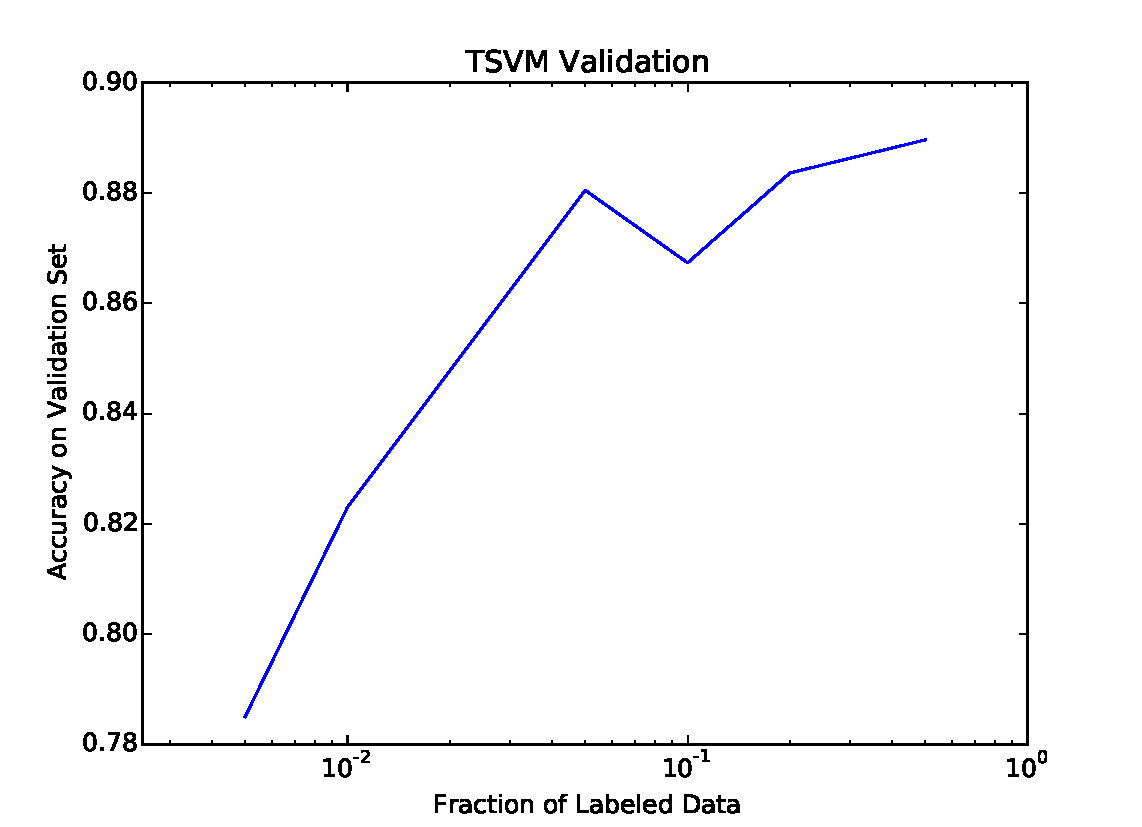
\includegraphics[width=5in]{tsvm.pdf}
\end{figure}

%[Insert comments about digits that the TSVM often mistook for another]

As can be seen from Table \ref{my-table}, certain pairs of digits were more likely to be confused by the algorithm. For example, a large number of 0's were classified as 8's and a large number of 1's as 5's, and a fair number of 9's as 1's. A likely explanation for why
some of the 0's were misclassified as 8 is that some instances of 0 were written with a slash through (like `$\emptyset$' as opposed to `0').

\section{Future Plans}

For future work, we plan to test the Spectral Graph Transducer algorithm described in section 3.2. We have also not yet incorporated the second data set from \cite{Llorens:2008}. We may end up deciding to not incorporate this data at all, since the data is in a different format and it has more symbols such as Latin letters and Unicode characters and there are fewer samples per character.

An additional aspect we would like to explore is trying different representations of our feature space (besides kernels). For example, instead of representing the individual points in $\mathbb R^2$, we replace the data with lengths of the segments between the points as well as the angle between segments (and perhaps also the initial orientation so that 6's and 9's are not confused).

Another area of exploration is trying different kernels for the TSVM, perhaps something more complex than a linear kernel and not as advanced as a Gaussian kernel. Doing feature selection could help us find a good kernel. For example, we could change the algorithm of \cite{Joachims:1999} by not enforcing exactly $num_+$ examples to be classified as +1. Another approach would be to use the Graph kernel methods of \cite{smola2003kernels}. We would also like to try different values for the parameters in the algorithm.

Another line of attack we seek to explore is implementing a semi-supervised deep neural net, perhaps one described by \cite{Lee:2013}. Lee's algorithm consists of a unsupervised phase, a supervised phase, and a semi-supervised phase. The first phase ignores the labels entirely and trains an autoencoder to get a better representation of the data. The second phase uses the labeled data to train the full network using gradient descent and dropout. For the final phase, Lee uses the method of \emph{pseudo-labels} to utilize more fully the unlabeled data. In this method, during each round of gradient descent, the neural net is trained on both kinds of data. The labeled data is treated as normally. For the unlabeled data, a classification is chosen based on most most highly activated output unit for the unlabeled data point, and the accuracy of the neural network on that data point is measured from the inferred classification.

\bibliographystyle{alpha}
\bibliography{midway}

\end{document}
